\documentclass[a4paper,12pt]{article}
\usepackage[T1]{fontenc}
\PassOptionsToPackage{defaults=hu-min}{magyar.ldf}
\usepackage[magyar]{babel}
\usepackage[a4paper]{geometry}
\geometry{margin=2cm}
\usepackage{listings}
\usepackage{graphicx}
\usepackage[table]{xcolor}
\usepackage{fancyhdr}
\usepackage{listingsutf8}

\begin{document}
	\pagestyle{fancy}
	\fancyhf{}
	\fancyhead[LE,RO]{\normalfont\normalsize\thepage}
	\fancyhead[RE]{\nouppercase{\sffamily\small\leftmark}}
	\fancyhead[LO]{\nouppercase{\sffamily\small\rightmark}}
	
	\title{{\Large Beadandó feladat} \\Bevezetés a kommunikációelméletbe  \\ {\small (LBG\_KM731K2)} \\[1cm] {\huge Eric Berne: Emberi játszmák}}
	
	\author{Kovács Norbert és Szabó Bence}
	
	\date{\today}
	\maketitle
	
	\newpage
	
	\section{Bevezetés}
	\subsection*{Eric Berne}
	Eric Berne, kanadai pszichiáter, aki leginkább a \textit{tranzakcióanalízis} kidolgozójaként, és az \textit{Emberi játszmák} című könyve révén vált híressé.
	Számomra Berne legérdekesebb és legfontosabb gondolata szerint a szervezetnek ingerlésre van szüksége a megfelelő funkcionáláshoz. Itt felmerül egy nagyon kifejező gondolat, hogy az ingerlés a legfontosabb, nem pedig a kellemes inger. Emiatt a gondolat miatt szerettem volna belevetni magam a munkájába, és elemezni az Emberi játszmák című könyvét.
	
	\subsection{Társas érintkezés}
	Az első, és legfontosabb gondolat a könyv első fejezetében, hogy a hanyagolás, és érzelmi nélkülözés leépüléshez vezet. Könnyedén párhuzamba hozható az ingeréhség, és a valódi táplálék éhség. 

	\begin{flushright}
		{\footnotesize 		,,Ha az agytörzs retikuláris aktiváló rendszerét nem éri elegendő inger,\\ akkor az idegsejtekben -- legalábbis közvetve -- elsorvadási folyamat indulhat meg. Előfordulhat, hogy ez a folyamat a rosszul tápláltság másodlagos hatása, de a hiányos táplálkozás maga is lehet az apátia terméke''}
	\end{flushright}

	Számomra ebből a legfontosabb tanulság, hogy közvetve, vagy közvetett módon mindenféleképpen egy leépülés követi az ingerszegénységet, és komoly egészségügyi és fizikai következményekkel kell számolnunk.
	
	Kifejező, hogy sok terminológiát áthelyezhetünk szinte egyenesen a táplálkozás területéről. Az ingeréhséget a táplálékéhséggel, a túltápláltságot a túlingerléssel stb. A könyv megemlít bizonyos fogalmakat amiknél nem fedi le a párhuzam másik oldalát, ami nagyon kíváncsivá tett.
	Megpróbáltam  megfogalmazni saját magam ezeket a párhuzamokat, de arra jutottam, hogy egy-egy kifejezésre, több párhuzam is hozható, és legtöbbször személyes, egyéni tapasztalat miatt fűzöm össze. 
	\begin{itemize}
		\item A megemlített \textit{ínyencséget} először a saját olvasási szokásaimmal hoztam párhuzamba, miszerint science fictiont, csak egy írótol vagyok ,,hajlandó'' olvasni. \\
		De ínyencségnek fogalmaznám meg azt is, amikor egy \textbf{konkrét}, \textbf{speciális} elismerési formára vágyik az ember egy szerepkörben. Pl.: ,,nagyon jó vezető vagy'', ,,nagyszerű oktató vagy''.
		\item Az aszkézist, a ki nem mondott igazsággal hoznám párhuzamba. Főleg egy olyan közegben ahol nagy ellenérzéseket, tompítást vált ki minden negatív gondolat, vagy ,,rossz'' dologra való figyelemfelhívás.
		\item A torkosságot a véget nem érő, élvezetes beszélgetések vágyával kötném össze, amikor olyan személlyel kommunikálunk akinek a véleménye hasonlatos a miénkkel, és ,,feltartjuk'' egymást. \\
		Számomra itt szintén megjelenik párhuzamként a ,,túltolod'' kifejezés. Az élet különböző területein való túlteljesítés véleményem szerint torkosság. Célja szerintem a túlzott elismerés kiváltása.
	\end{itemize}
	Ezen a ponton úgy gondolom, hogy a hozott párhuzamok teljesen személyes tapasztalatokra épülnek, és az hogy egy pontra több párhuzam is megjelent, annak a jele hogy nem elég általános az értelmezésem. Ettől függetlenül kifejezetten érdekes gondolatnak tartom, hogy az étkezési szokásainkat ilyen szerepkörben is lehet használni.
	
	El szoktuk fogadni a gondolatot hogy ,,nem tehetek róla hogy éhes vagyok, ennem kell''. Viszont nagyon nehéz kimondani hogy ,,törődésre van szükségem, szeressetek''. Pedig mind a kettő érzés, eszerint a megközelítés szerint rajtunk kívülálló szükségletünk, még is máshogy kezeljük.
	
	Ennek a feloldása nálam ott történt meg, amikor megemlítjük a rejtett, jelképes gondozási formákat. Mivel nehéz kijelentenünk, vagy megfogalmaznunk ezeket a szükségleteinket, \textit{kompromisszumokat} kötünk a társadalommal. Megjelennek a jelképes gondozási formák. A könyv példája szerint, egy színésznek hetente akár 100 ,,simogatásra'' is szüksége van, amíg egy tudósnak évente elég egy simogatás is a megfelelő szakmai vezetőtől.
	
	\begin{flushright}
		{\footnotesize 		,,A \textit{simogatást} az intim fizikai kapcsolat általános fogalmának értelmében használjuk; a gyakorlatban ez különféle formákat  ölthet.\\ \dots \\ 
		A \textit{simogatás}  fogalmát, jelentésbővítéssel, köznyelvileg minden olyan aktus jelölésére alkalmazhatjuk, amely egy másik személy jelenlétét nyugtázza.''}
	\end{flushright}

	Ennek a fejezetnek az utolsó gondolata valahol nagyon meglepett. A konklúzió hogy a gyengéd törődés és az áramütés is pozitív hatású, amíg a hanyagolás káros (egérkísérletek során).
	Úgy gondolom hogy ez egy olyan erős alapja a bántalmazó kapcsolatoknak, ami kissé új fénybe borítja a bántalmazott szerepkört. Ha ennyire mélyen rejtőzik az, hogy a bántalmazás is jobb mint a hanyagolás, és megjelenik a ,,legalább foglalkozik velem'' kifejezés, valójában bármilyen aspektusból hibáztatható-e a bántalmazott? (Sokszor megjelenik az a motívum, hogy a bántalmazott hagyja magát, és ő is tehet róla) Egy sokkal vitathatóbb kérdés, hogy mennyire hibáztatható a bántalmazó ebben a szerepkörben. Lehetséges, hogy sok esetben a bántalmazó ezt törődési formának érzékeli. Sokszor elhangozhat az a mondat, hogy ,,addig jó amíg veszekszek, mert az azt jelenti hogy még érdekel''. Az intenzív veszekedés, és nem vita, alapvetően romboló jellegű a véleményem szerint, mégis sokan ezt elfogadható eszköznek érzik a törődés kifejezésére, és eszerint a megközelítés szerint, nem is tévednek nagyot.
	

	\subsection{Az idő strukturálása}
	Mindenkinek feladata és felelőssége az ébrenlét órát strukturálni, hogy eleget tegyen a struktúra éhségének. Berne megfogalmazásában az idő strukturálását nevezhetjük programozásnak, és ezt három csoportra bontja: \textit{anyagi}, \textit{társadalmi} és \textit{egyéni}.
	
	A könyvben elhangzik egy hasonlat, a hajóépítés dinamikájáról. A hajóépítők csoportjának minden társas érintkezésüket alá kell rendelniük az előre megszabott munkafolyamatoknak, mert csak így haladhat előre a hajó építése. Az \textit{anyagi programozás} forrása a külső valósággal való megbirkózás, lényegében az adatfeldolgozás az alapja.
	
	A \textit{társadalmi programozás} egy sokkal érdekesebb csoport. Ide a hagyományos, rituális vagy fél rituális érintkezéseket soroljuk. Ezeket az érintkezéseket nevezhetjük jó modornak, amit szüleinktől tanulunk meg, és nagyon változatosak lehetnek. 
	
	\begin{flushright}
		{\footnotesize 		,,Helyi, ősi hagyomány bátorítja  vagy  tiltja,  lehet-e  böfögni  az  étkezésnél,  lehet-e érdeklődést tanúsítani  más felesége  iránt. E két sajátságos 	tranzakció  között például fordított kölcsönösségi viszony figyelhető meg: rendszerint nem tanácsos az asszonynép után érdeklődni  ott,   ahol  az  emberek    böfögnek  étkezés  után; olyan  helyeken  viszont,  ahol  lehet az asszonynép után érdeklődni, ott nem tanácsos étkezéskor böfögni.''}
	\end{flushright}

	Berne szerint amikor két ember közelebbről megismeri egymást, egyre több \textit{egyéni programozás} csúszik be. Ezek afféle incidensek, viszont egyértelműen mintát követnek, csoportosíthatóak és osztályozhatóak.
	
	Ezek az időtöltések és játszmák, a valódi intimitás pótlékai. A valódi intimitás akkor kezdődik el, amikor az egyéni programozás intenzívebbé válik mint a társadalmi szabályozás. 
	
	\begin{flushright}
		{\footnotesize 	Az intimitás az egyetlen tökéletesen kielégítő válasz az ingeréhségre,  az  elismeréséhségre  és  a  struktúraéhségre. Prototípusa a szerelmi egyesülés.}
	\end{flushright}

	Az idő strukturálásának célja az unalom, magány elkerülése. Csoportban is lehet valaki magányos, viszont egy csoportban több lehetőségünk nyílik az idő strukturálására. A csoportosulás tagjainak célja, hogy a többiekkel lebonyolított tranzakciókból a lehető legtöbb kielégüléshez jussanak. Fontos, hogy a kielégülés szót nehéz egyértelműen értelmezni, mert sok ilyen tranzakció önpusztító jellegű, ezért Berne a nyereség, vagy előny szavakat használja ezentúl.
	
	Az idő strukturálását  feloszthatjuk rituálékra, időtöltésekre, játszmákra, intimitásra és tevékenységekre. Úgy a társas érintkezésből származó nyereségeink, feszültségcsökkenésre, ártalmas helyzetek elkerülésére, a simogatásunk megszerzésére, és az egyensúly fenntartására oszthatóak.
	
	A legfontosabb hogy ezeket sokkal hasznosabb előnyként vizsgálni, mint védekezésként. Ugyanis a legjobb védekezés, ha nem folytatunk semmilyen tranzakciót, és a védekezés nem is fedi le teljesen az említett szempontokat.

	\section{Játszmaelemzés}
	\subsection{Strukturális elemzés}
	
	Ebben a fejezetben az \textit{én-állapotok} fogalmába kapunk részletesebb betekintést. Köznyelvi megnevezésükön: szülői, felnőtti, gyermeki én-állapot. Mindenki egy adott pillanatban, valamelyik én-állapotot engedi megnyilvánulni.
	
	Először, én úgy gondoltam, hogy egy egészséges személyiség esetén a Felnőtti én-állapotnak kell uralkodnia, viszont rosszul hittem. Minden én állapotnak kritikusan fontos szerepe van a hétköznapokban.
	\begin{itemize}
		\item A Gyermekben intuíciók, kreativitás, alkotókészség, spontán hajtóerők és örömök jelennek meg. Én ezt úgy értelmezem, hogy a bennünk rejlő gyermek éli meg örömeinket, talál ki innovatív megoldásokat.
		\item A Felnőtt a fennmaradáshoz elengedhetetlen. Számításokat, adatelemzést végez, a segítségével birkózunk meg a világ problémáival, és feladatainkkal. A Felnőtt szerzi meg a tapasztalatokat, például arról mi nyújt örömöt vagy kudarcot. A Felnőttnek még az is feladata hogy szabályozza a Szülő és Gyermek tevékenységét, és tárgyilagosan közvetítsen. Számomra a megfontolt, mérlegelt objektív szemléletet képviseli a Felnőtt.
		\item A Szülő elsődleges funkciója, a konkrét, valóságos gyermekek nevelése. Ezenkívül bizonyos folyamatokat, és válaszokat automatikussá tesz. Ezzel rengeteg ,,számítást'', időt és energiát spórol meg a Felnőttnek. Számos dolog megszokás kérdése, és nem kell a Felnőttnek apróbb ügyekben is ,,intézkednie'', a rutinügyeket a Szülőre bízza.
	\end{itemize}
	Számomra kifejezetten érdekes, hogy ezeknek az én állapotoknak a szerepköre kiegyensúlyozott kell hogy legyen, és problémák akkor jelenhetnek meg, amikor valamelyik én-állapot túlnyomóan uralkodik. Fontos, hogy a ,,gyerekes'' szónak olyan negatív mellékzöngéi vannak, ami miatt ez esetben nem is használunk. Úgy gondolom, hogy amikor valaki a Gyermek én-állapotot engedi érvényesülni, egy olyan szituációban, ahol a Felnőtt, analitikus én-állapotra lenne szükség, ekkor fogalmazódik meg bennünk valakiről hogy gyerekes. Viszont látnunk kell, hogy a Gyermek ugyan olyan nagy szerepkörrel rendelkezik mint a másik két én-állapot.
	
	Ezek az én-állapotok teljesen elkülönülnek egymástól, sokszor egymással ütköznek is, mégis egy családon belül szerintem ezek egy láncolatot alkothatnak. Tudjuk hogy hatással vagyunk egymásra, és ,,alakulunk'' szeretteinkhez, barátainkhoz. A valódi szülő-gyermek kapcsolat esetén, véleményem szerint hozható párhuzam az én állapotok között. (A szüleink Felnőtt, és a mi Szülő én-állapotunk szerintem szoros kapcsolatban állnak)
	
	A Gyermeki én állapot megfogalmazása szerint, mindig voltunk fiatalabbak magunknál, ezért van olyan korábbi pillanat, ahonnan hozhatunk magunkkal rögzült maradványokat, amik előhozhatóak. 
	Mindenki képes objektíven szemlélni a valóságot (beleértve a gyermekeket, értelmi fogyatékosakat, vagy szkizofréneket is), tehát mindenkiben lakozik egy Felnőtt. És mindannyiunknak megvannak a saját szüleink vagy szülőpótlékaink, ahonnan újratermelhetjük a szülők/szülőpótlékok én-állapotait. 
	
	\subsection{Tranzakcionális elemzés}
	Ez a fejezet a társas érintkezés folyamatairól szól, egy kifejezetten erős eszköz a különböző konfliktusaink megértéséhez, és kezeléséhez. Nevezzük a társas érintkezés egységét tranzakciónak. Valamilyen társas érintkezés során, amikor beszélgetést kezdeményezünk, tranzakcióst ingerként szolgálunk. Amennyiben valamilyen módon ezzel kapcsolatos reakció történik, azt tranzakciós válasznak nevezzük.
	
	Itt az én-állapotok közötti tranzakciók a hangsúlyosak. Kijelenthető, amennyiben ,,párhuzamos'' az én-állapotok közötti tranzakció, addig minden rendben. Ez alatt azt értem, hogy ha Felnőtt-Felnőtt tranzakció történik az én részemről, azt várom el, hogy Felnőtt-Felnőtt válasz érkezzen. Ezt legjobban a következő ábra szemlélteti: \\[0.3cm]
	
	\begin{center}
		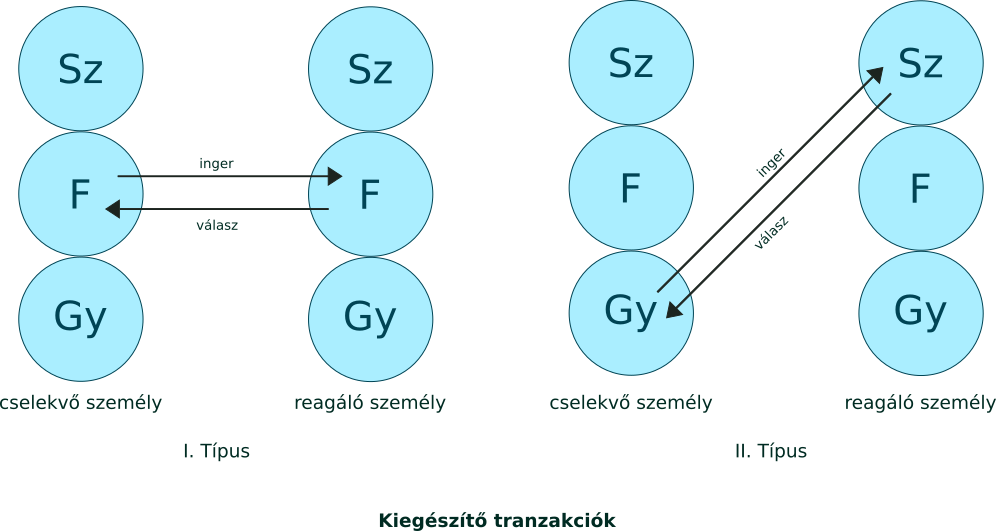
\includegraphics[width=15cm]{svgs/parhuzamos_tranzakciok.png} \\[0.5cm]
	\end{center}
	Fontos látnunk hogy minden válasz, maga egyben inger is lehet, így a tranzakció a végtelenségig is folyhat. Ezt nevezzük gördülékeny tranzakciónak, vagy ahogyan én nevezném, párhuzamos tranzakciónak, ugyanis az én-állapotok egymásra reagálva, párhuzamosan céloznak meg egy-egy én-állapotot. Amint megtörik a párhuzamosság, kezdődnek a problémák a tranzakciókban. Azaz, a kommunikáció keresztezett tranzakció esetén megszakad.
	
	Itt fontos hangsúlyt fektetni arra, hogy a kommunikáció szakad meg, nem pedig maga a tranzakció. Ilyenkor szoktak megjelenni a köznyelvből hallható, ,,elbeszélnek egymás mellett'', vagy a ,,elcsúszott a kommunikáció''. Tehát, a két fél információcseréje szakad meg. Továbbra is fennáll a kísérlet arra mind a két fél részéről hogy kommunikáljanak, de mivel rossz a ,,címzett'', ezért az feszültséget, konfliktust szül.
	
	\begin{center}
		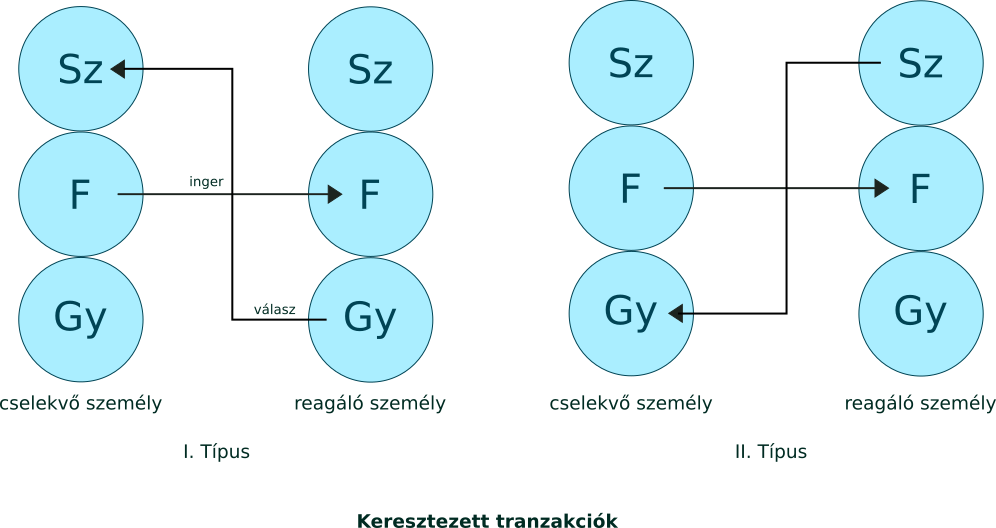
\includegraphics[width=15cm]{svgs/keresztezett_tranzakciok.png} \\[0.5cm]
	\end{center}
	Ennek a megoldása az, hogy korrigáljuk a párhuzamosságot. Vagy a cselekvő fél vált át a megfelelő szerepkörbe, vagy a reagáló személy vált az eredetileg megcélzott én-állapotba. Ez az adott konfliktustól függően sikerülhet azonnal, vagy egyáltalán nem.
	
	Itt számomra az első felmerülő kérdés, miután megpróbáltam értelmezni a kereszteződés lényegét, hogy hogyan kellene kezelnünk a ,,fél-kereszteződő'' tranzakciókat. Az értelmezésem szerint gördülékenyen zajlik egy tranzakció egészen addig, amíg az párhuzamos, avagy kiegészítő, és ahol a válasz egyben inger is. 
	Ezzel ellentétben, amennyiben a fent szemléltetett kereszteződés fellép, azonnal érezzük egy konfliktus megjelenését, akár sértődöttséget, vagy lekezeltséget. Sok a közelünkben zajló konfliktust rátudunk tenni erre a modellre, és azonnal látni fogjuk hogy a kiváltó ok valóban a keresztezett tranzakciókból ered. 
	
	A könyv 9 különböző interakciót vázol fel, ahol jól láthatóak a kereszteződések, és párhuzamok. Fél-kereszteződő tranzakciónak azokat a tranzakciókat értem, ahol nem a megcélzott én-állapot válaszol, de annak az én-állapotnak ahonnan az inger indult. Ezt nem nevezhetjük kereszttranzakciónak, mivel nincs kereszteződés, viszont számomra érdekes kérdés hogy ez pontosan mit jelent, vagy egyáltalán probléma-e. \\[0.3cm]
	\begin{center}
		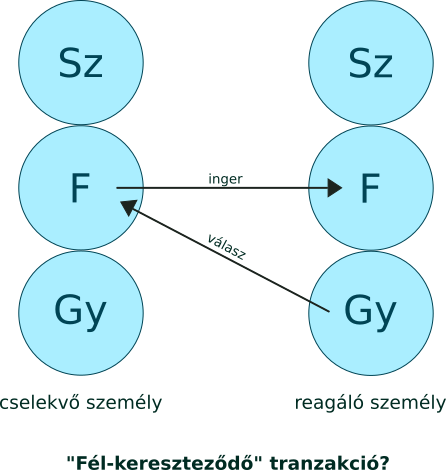
\includegraphics[width=7cm]{svgs/fel_keresztezodo_tranzakciok.png} \\[0.8cm]
	\end{center}
	Erre a kérdésre adhat választ a rejtett tranzakció. Sokkal összetettebb, egyidejűleg kettőnél több én-állapotot von be. A könyv egy példát hoz egy kereskedőről:
	\begin{itemize}
		\item Kereskedő: ,,Ez itt jobb, de maga ezt aligha engedheti meg magának.''
		\item Háziasszony: ,,Márpedig ezt fogom megvenni.''
	\end{itemize}
	Azt gondolhatnánk, hogy a Kereskedő Felnőtt én-állapota szólt a Háziasszony Felnőtt én-állapotához, hiszen tényt szögez le, ,,Ez itt jobb'', és ,,Maga ezt aligha engedheti meg magának''. Azonban a Felnőtt válaszának úgy kellene szólnia, hogy; ,,Mindkét dologban igaza van''.
	Azonban érezzük hogy a Kereskedő nem teljesen a Felnőttnek célozta az üzenetet, hanem a Gyermeknek, amire a Háziasszony Gyermeke válaszolt is. Mégpedig: ,,Fütyülök az anyagi következményekre, megmutatom én ennek a fickónak''.
	Érdekes számomra hogy a szöget bezáró kommunikáció esetén érzünk egy feszültséget, valamiféle konfliktust, vagy lekezelést, mégis kiegészítő tranzakcióról van szó, mert a megfelelő én-állapotok között bizony meg van a kapcsolat.
	
	Ezen kívül a dupla fenekű rejtett tranzakcióban négy én-állapot vesz részt, többnyire flörtjátszmákban fordul elő. A könyv által hozott példa:
	\begin{itemize}
		\item Tehenészfiú: ,,Jöjjön, nézze meg az istállót!''
		\item Lány: ,,Kislány korom óta imádom az istállókat''
	\end{itemize}
	Alapvetően egy Felnőtt társadalmi szinten folyó beszélgetés folyik az istállókról, pszichológia szinten pedig Gyermek beszélgetés a szerelmi együttlétről. Mind a két oldalról párhuzamos a tranzakció, hiszen a Felnőtt a Felnőttet célozza meg az istállók szépségéről, és megfelelően célzott választ is kap. Gyermek szinten megjelenik a ,,gyere játszunk'' üzenet, ami ebben az esetben párhuzamos tranzakcióval ,,elfogadásra'' kerül, és a körülményektől függően sejthetjük a történet folytatását.
	
	
	
	\begin{center}
		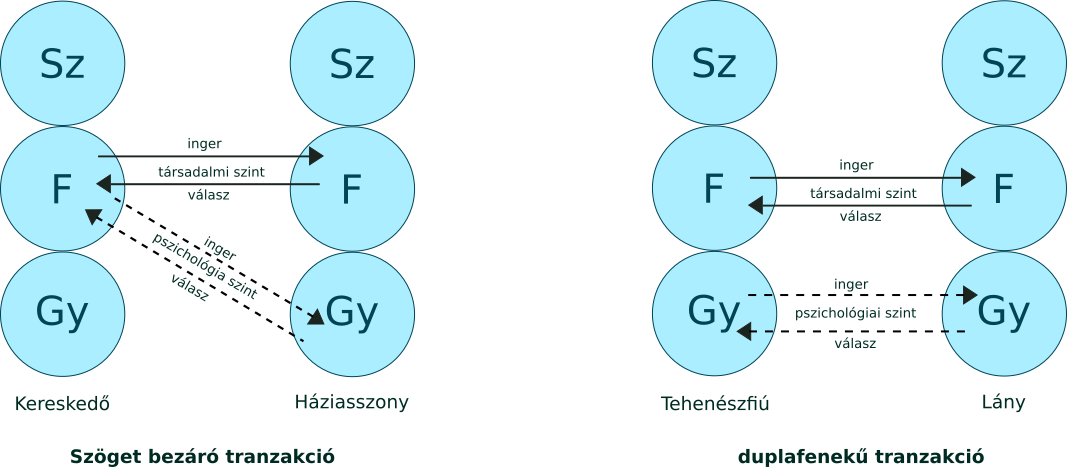
\includegraphics[width=15cm]{svgs/rejtett_tranzakciok.png} \\[0.5cm]
	\end{center}

	Berne nem tér ki arra, hogyan jellemezhető az, amikor a rejtett tranzakció is kereszttranzakcióvá válik. A később szemléltetett ábrán a Rejtett, és a Keresztezett azonos szinten helyezkedik el. Számomra felmerül a kérdés, hogy vajon előfordulhat hogy a rejtett tranzakció ,,sikertelen'', vagy keresztezett?
	
	Mire gondolok akkor amikor a rejtett tranzakció esetén kereszteződést vélek felfedezni?
	Az előző példával élve, mi történik akkor, ha a Tehenészfiú rejtett ajánlatát a szerelmi együttlétre, elutasítás követi? Azt tudjuk, hogy rejtett szinten a Gyermek kérte fel ,,játszani'' a lány Gyermekét. Az egyszerű elutasító válasz szintén jöhet a Gyermektől, ezért ott ugyan így tudnánk ábrázolni az interakciót. Az esetben, ha a Felnőtt válaszolna, rejtett tranzakcióval, mégpedig valahogy úgy, hogy ,,Nagyon késő van, otthon kell lennem'', akkor ez tekinthető-e kereszteződésnek? Valójában ez társadalmi szinten  egy Felnőtt reakció, tényt közöl, tehát eddig minden rendben. Pszichológia szinten, tekinthetjük-e ezt Felnőtt tranzakciónak a ,,kérlelő'' Gyermek felé, ami egy elutasítása a szerelmi együttlétnek? Hogy ha elfogadjuk, hogy a Felnőtt reakciója, akkor is csak Szöget bezáró tranzakcióról van szó.
	Úgy gondolom, hogy akkor fordulhat elő kereszt tranzakció, ha a leány Szülője reagál a rejtett tranzakció során.
	
		\begin{center}
		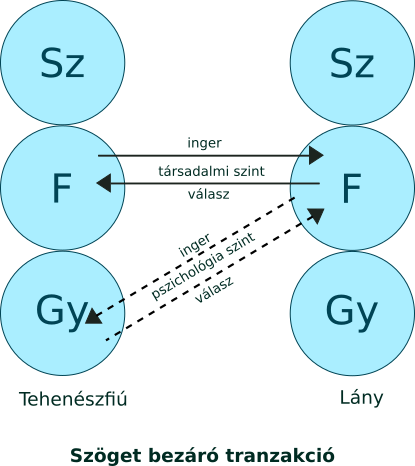
\includegraphics[width=6cm]{svgs/kereszt_tehenesz_tranzakcio.png} \\[0.5cm]
	\end{center}
	Itt az a megérzésem, hogy nem a rejtett elutasítás teszi lehetővé a kereszt tranzakciót, ahogyan az először gondoltam, hanem az hogy a lány Szülő én-állapota reagáljon rejtett tranzakcióval. Ezen gondolkodva, azonban nem tudtam olyan példát/reakciót találni ami társadalmi szinten Felnőtt, de rejtett szinten Szülői én-állapot. Nyilvánvalóan oka van annak hogy Berne nem tért ki erre, és én sem jutottam válaszra a saját kérdésemet illetően. Azért tartom fontosnak megemlíteni, ezt a ,,sikertelen'' gondolatmenetet, mert úgy vélem hogy nem elegendő elfogadnunk mások kijelentéseit, még az esetben sem ha kiváló szakemberekről van szó, de körbe kell járnunk a témát a saját kérdéseinkkel, még akkor is, ha végül pontosan ugyan arra a konklúzióra jutottunk mint az író. 


	Berne a következő rendszerbe osztja a tranzakciókat, ezzel zárva a fejezetet:\\[0.2cm]

	\begin{center}
		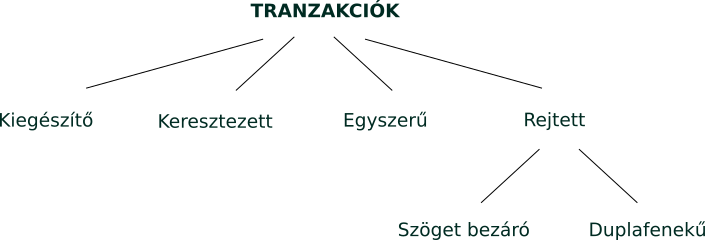
\includegraphics[width=13cm]{svgs/tranzakciok.png} \\[0.5cm]
	\end{center}

	\section{Összegzés}
	A könyv csupán első két fejezetét sikerült feldolgoznunk, és a konkrét játszmákra ki sem tértünk. Nem szerettem volna csupán felületesen betekinteni a játszmák leírásába, és ezzel egy túlságosan felszínes képet adva a témáról. Úgy vélem, hogy a könyv első két fejezete is mély vitaindító lehet, és további gondolatok szülője. A legfontosabb hozadéka véleményem szerint ennek az első két fejezetnek, hogy megértsük az én-állapotokat. Fogalomtisztázás után, (A Gyermek nem gyerekes, a Felnőtt nem komor, a Szülő nem atyáskodó) kifejezetten erős eszköz konfliktus kezeléshez. Mindennapi interakcióink társainkkal, tranzakcióink során rengeteg konfliktusba ütközünk. Rengetegszer kimarad az empátia ezekből a tranzakciókból, és feszültségek gyülekeznek, amik hosszútávon épülhetnek, és tovább rombolhatják szociális kapcsolatainkat.
	
	Ha új megfogalmazásba kellene tennem az empátiát ezek szerint a gondolatok szerint, akkor azt mondanám, hogy az empátia, az a képességünk, amivel korrigálni tudjuk tranzakcióink párhuzamosságát, mégpedig úgy hogy megértjük a társunk üzenetét, és helyzetét.
	
	Amennyiben az ilyen konfliktusokból picit elemzőbb szemmel tudunk kilépni, talán könnyebben a megoldás útjára tudunk majd lépni. Például a szerepváltás véleményem szerint nehéz feladat, és jól kell megfigyelnünk, hogy az inger melyik én-állapotunknak szólt, de ha sikerül, akkor saját magunknak is megkönnyítjük a tranzakciókat, csökkentjük a sértődés, vagy feszültségek megjelenésének esélyét, akár fogadó, vagy cselekvő szerepkörben legyünk.
	
	A könyv megfogalmazta, hogy a tompítás tapintat, az erősítés diplomácia érzék. Számomra ez egy érdekes megközelítés, és úgy gondolom, hogy mindkettőre szükség van a természetes társas tranzakcióink során. Véleményem szerint, az sem feltétlenül gond, hogy ha két személy külön reprezentálja a tapintatot, és a diplomáciai érzéket, és ezek ütköznek egymással. Egészen addig, amíg a két oldal egyenlő félként szerepel, nincs alá-fölé rendeltség, és fennáll az egyensúly a tranzakció során, és lehetőleg párhuzamos/kiegészítő tranzakcióról van szó.
	
	Úgy gondolom hogy ha törekszünk a kiegészítő tranzakciókra, és tudatosan kezeljük a kereszttranzakciókat, tisztában vagyunk a rejtett tranzakciók fontosságával, sokkal kevésbé reagálunk érzelmi alapon a különböző élethelyzetekre, ezzel is közelebb kerülve a hajó megépítéséhez.
	
	\begin{center}
		
\includegraphics[width=11cm]{svgs/ship.png} \\[0.5cm]
	\end{center}
	
\end{document}